Součástí této práce jsou i tři ukázkové aplikace, které jsem vytvořil pomocí frameworku PhoneGap a slouží jako základní seznámení autora práce s frameworkem a také jako demonstrace použití základních API volání, které framework poskytuje.

\section{Twitter klient (BlueBirdGap)}
První aplikací, kterou jsem ve frameworku PhoneGap vytvořil, je jednoduchý klient pro sociální síť Twitter. Obsahuje pouze elementární funkce, kdy se může uživatel přihlásit svým uživatelským jménem a heslem, zobrazit svojí timeline a také odeslat na Twitter nový tweet. Aplikace byla původně zamýšlena jako multiplatformní, tedy tak, aby se dalo co možná největší množství kódu použít i na dalších platformách. Nakonec jí bylo z důvodu platformní závislosti pluginu ChildBrowser možné využít jen na platformě Android.

V průběhu vývoje jsem narazil na problémy zejména s implementací otevřeného protokolu OAuth, který je vyžadován k autentizaci uživatele na Twitteru. Implementace tohoto protokolu pomocí JavaScriptu není přímočará záležitost, neboť tento postup skýtá bezpečnostní rizika v podobě odhalení přenášených bezpečnostních klíčů. Nakonec jsem využil knihovny jsOAuth, která nabízí abstraktní rozhraní pro využití tohoto protokolu. K tvorbě uživatelského rozhraní jsem využil framework jQuery Mobile spolu s vlastními CSS styly.

\begin{figure}[htbp]\centering
\includegraphics[width=0.8\textwidth]{bbgap_timeline_2.png}
\caption{BlueBirdGap, zobrazení timeline}
\label{fig:BbGapTimeline}
\end{figure}

Pokud se zaměříme na unikátní vlastnosti frameworku PhoneGap, které byly v této aplikaci využity, musím na prvním místě uvést oficiální plugin ChildBrowser, který umožňuje v rámci WebView otevřít další WebView jako svého potomka. Této funkce bylo využito při identifikaci uživatele, kdy se mu otevře jako potomek další okno, kde musí ověřit své přihlašovací údaje na webové stránce Twitteru. Z dalších funkcí uvedených v API PhoneGap můžu zmínit například využití místní databáze localStorage pro uložení údajů o konkrétním uživateli.

Aplikace byla otestována v Android emulátoru na verzi systému 4.2.

\section{Foto aplikace (Orionids)}
V druhé aplikaci jsem chtěl vyzkoušet patrně nejpřitažlivější funkci frameworku PhoneGap, za kterou pokládám možnost jednoduše ovládat fotoaparát daného mobilního zařízení. Vytvořil jsem za tímto účelem jednoduchou aplikaci, jejímž účelem je fotografovat a ukládat obrázky padajících hvězd. Zároveň s vyfocením fotografie je zaznamenána i geografická poloha místa, kde byla fotografie pořízena. Aplikace umožňuje pořídit fotografii buď přímo či jí vybrat z nativní galerie. Všechny fotografie jsou v aplikaci uložené a je možno zobrazit jejich přehled a také si prohlédnout detail každé z nich.

Protože byl pro tvorbu uživatelského rozhraní použit framework jQTouch, který je závislý na jádře WebKit, funguje tato aplikace pouze na platformách Android a iOS. Pro uživatelské rozhraní jsem využil předpřipravených šablon frameworku jQTouch, které se automaticky přizpůsobí platformě, na které běží, aby více simulovaly vzhled nativních aplikací. Finální vzhled jsem upravil vlastními CSS styly. Pro zobrazení míst, kde byly fotografie pořízeny, je využito vložené Google mapy s vyznačením dotyčných poloh.

\begin{figure}\centering
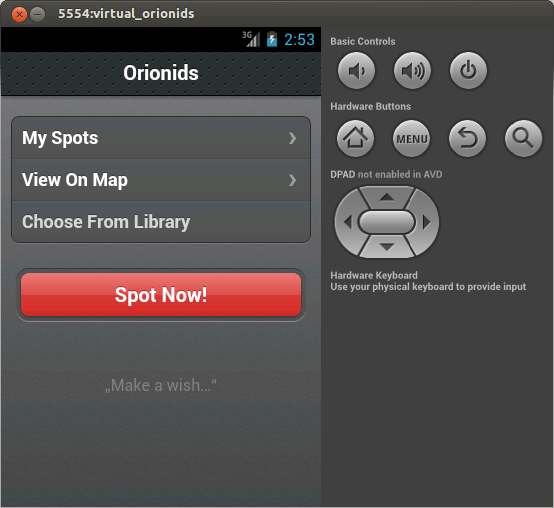
\includegraphics[width=0.8\textwidth]{orionids_home.png}
\caption{Orionids, domovská obrazovka}
\label{fig:OrionidsHome}
\end{figure}

V rámci této aplikace bylo rovněž využito několik API volání, které vývojářům nabízí framework PhoneGap. Stěžejním bylo pochopitelně využití API volání Camera, které umožňuje pořídit fotografii fotoaparátem či ji vybrat z nativní fotogalerie daného zařízení. Pro ukládání informací o pořízených fotografiích jsem využil volání Storage, které zpřístupňuje ukládání do lokální databáze dle specifikace konsorcia W3C. V neposlední řadě jsem využil volání Geolocation, které zpřístupňuje údaje o zeměpisné šířce a délce místa, kde se dané zařízení právě nachází. Na závěr musím podotknout, že používání všech API bylo velmi přímočaré a bezproblémové.

Aplikace byla otestována v Android emulátoru na verzi systému 4.2.

\section{Časovací aplikace (TimerGap)}
Poslední aplikací je jednoduchý časovač, který umožňuje uživateli spustit odpočítávání času využitelné například jako kuchyňská minutka pro odměření doby potřebné pro vylouhování čaje. Aplikace umožňuje spustit rychlé odpočítávání, uložit a pojmenovat odpočítávání pro další použití a samozřejmě vybírat a spouštět již uložené časy.

V této aplikaci jsem opět využil JavaScriptový framework jQuery Mobile, pomocí nějž jsem vytvořil uživatelské rozhraní a také využil jeho funkcí při tvorbě funkční logiky celé aplikace. Pro realizaci vlastního odpočítávání jsem využil knihovnu jQuery Countdown, která poskytuje pro jeho implementaci velmi podařené abstraktní rozhraní. Pro zajištění uživatelsky přívětivého způsobu vybírání času jsem využil plugin jQuery Mobile - Datebox.

\begin{figure}[htbp]\centering
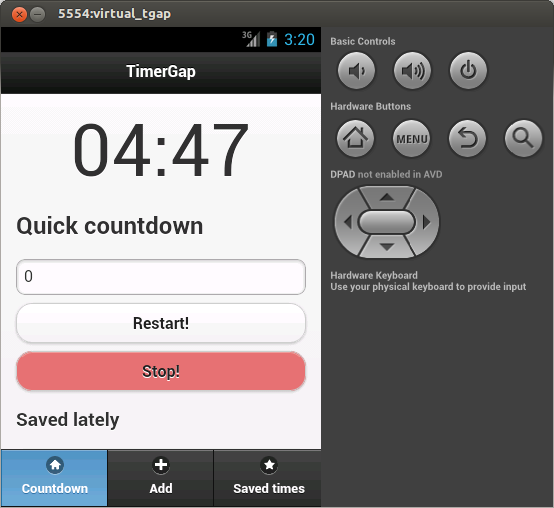
\includegraphics[width=0.8\textwidth]{tgap_odpocitavani.png}
\caption{TimerGap, proces odpočítávání}
\label{fig:TGapOdpocitavani}
\end{figure}

V této aplikaci jsem se zaměřil především na otestování notifikačních schopností frameworku PhoneGap, který nabízí několik možností jak upozornit uživatele na nějakou událost. Z rozhraní Notification  jsem využil téměř všechny nabízené možnosti: dialogy alert či confirm a v momentě vypršení odpočítávaného času také zvukové upozornění beep spolu se zavibrováním vibrate. Pro ukládání uživatelem definovaných odpočítávání jsem využil databázi localStorage.

Práce s výše zmíněnými API voláními byla poměrně bezproblémová, krom platformy Windows Phone 7, kde jsme narazil na problémy s databází localStorage, která se nad jádrem prohlížeče IE 9 chová poněkud nestandardně.
        
Aplikace byla otestována v Android emulátoru na verzi systému 4.2 a na mobilním telefonu Nokia Lumia 800 se systémem Windows Phone 7.8.